\usetikzlibrary{calc}
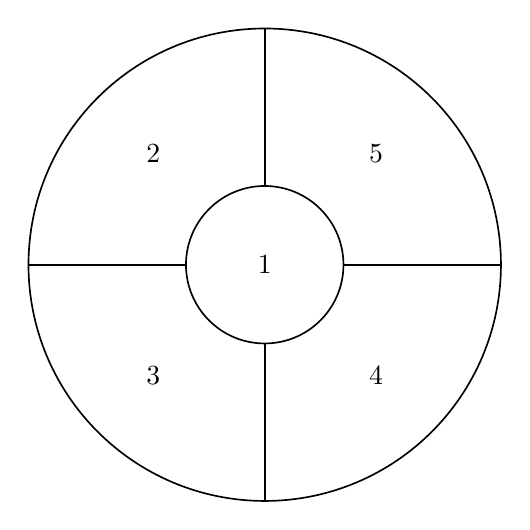
\begin{tikzpicture}[x=1cm,y=1cm,line width=.6pt,font=\normalsize]
\coordinate (O) at (0,0);
\draw (O) circle[radius=3];
\draw (O) circle[radius=1];
\draw (1,0) -- (3,0);
\draw (0,1) -- (0,3);
\draw (-1,0) -- (-3,0);
\draw (0,-1) -- (0,-3);
\node[inner sep=0pt,anchor=center] at (0,0) {$1$};
\node[inner sep=0pt,anchor=center] at (-1.4142,1.4142) {$2$};
\node[inner sep=0pt,anchor=center] at (-1.4142,-1.4142) {$3$};
\node[inner sep=0pt,anchor=center] at (1.4142,-1.4142) {$4$};
\node[inner sep=0pt,anchor=center] at (1.4142,1.4142) {$5$};
\end{tikzpicture}
